\justify

\section{Arquitecturas híbridas en sistemas distribuidos}

Las arquitecturas híbridas representan un enfoque de diseño de software que combina distintos estilos arquitectónicos dentro de un mismo ecosistema computacional con el objetivo de aprovechar las fortalezas de cada modelo. En sistemas distribuidos modernos es común integrar arquitecturas de microservicios con patrones internos de separación por capas, permitiendo desacoplar tanto los servicios como la lógica interna de cada componente.

Este enfoque favorece la modularidad, la mantenibilidad y la escalabilidad del sistema, ya que cada servicio puede operar de forma independiente mientras mantiene una organización estructurada de sus responsabilidades internas. Asimismo, la combinación de múltiples patrones arquitectónicos permite construir sistemas capaces de adaptarse a entornos de alta concurrencia y procesamiento distribuido.

\subsection{Arquitectura de Microservicios}

La arquitectura de microservicios es un enfoque de desarrollo de software en el que una aplicación se descompone en un conjunto de servicios pequeños, autónomos y altamente cohesionados. Cada servicio representa una capacidad funcional específica y se ejecuta como un proceso independiente, comunicándose con otros componentes mediante mecanismos ligeros, generalmente APIs REST sobre HTTP \cite{31}.

A diferencia de las arquitecturas monolíticas tradicionales, donde todos los módulos forman parte de una única unidad de despliegue, los microservicios permiten desacoplar funcionalidades y distribuirlas de forma independiente. Esta separación reduce el impacto de los cambios internos y facilita la evolución progresiva del sistema.

\begin{figure}[H]
    \centering
    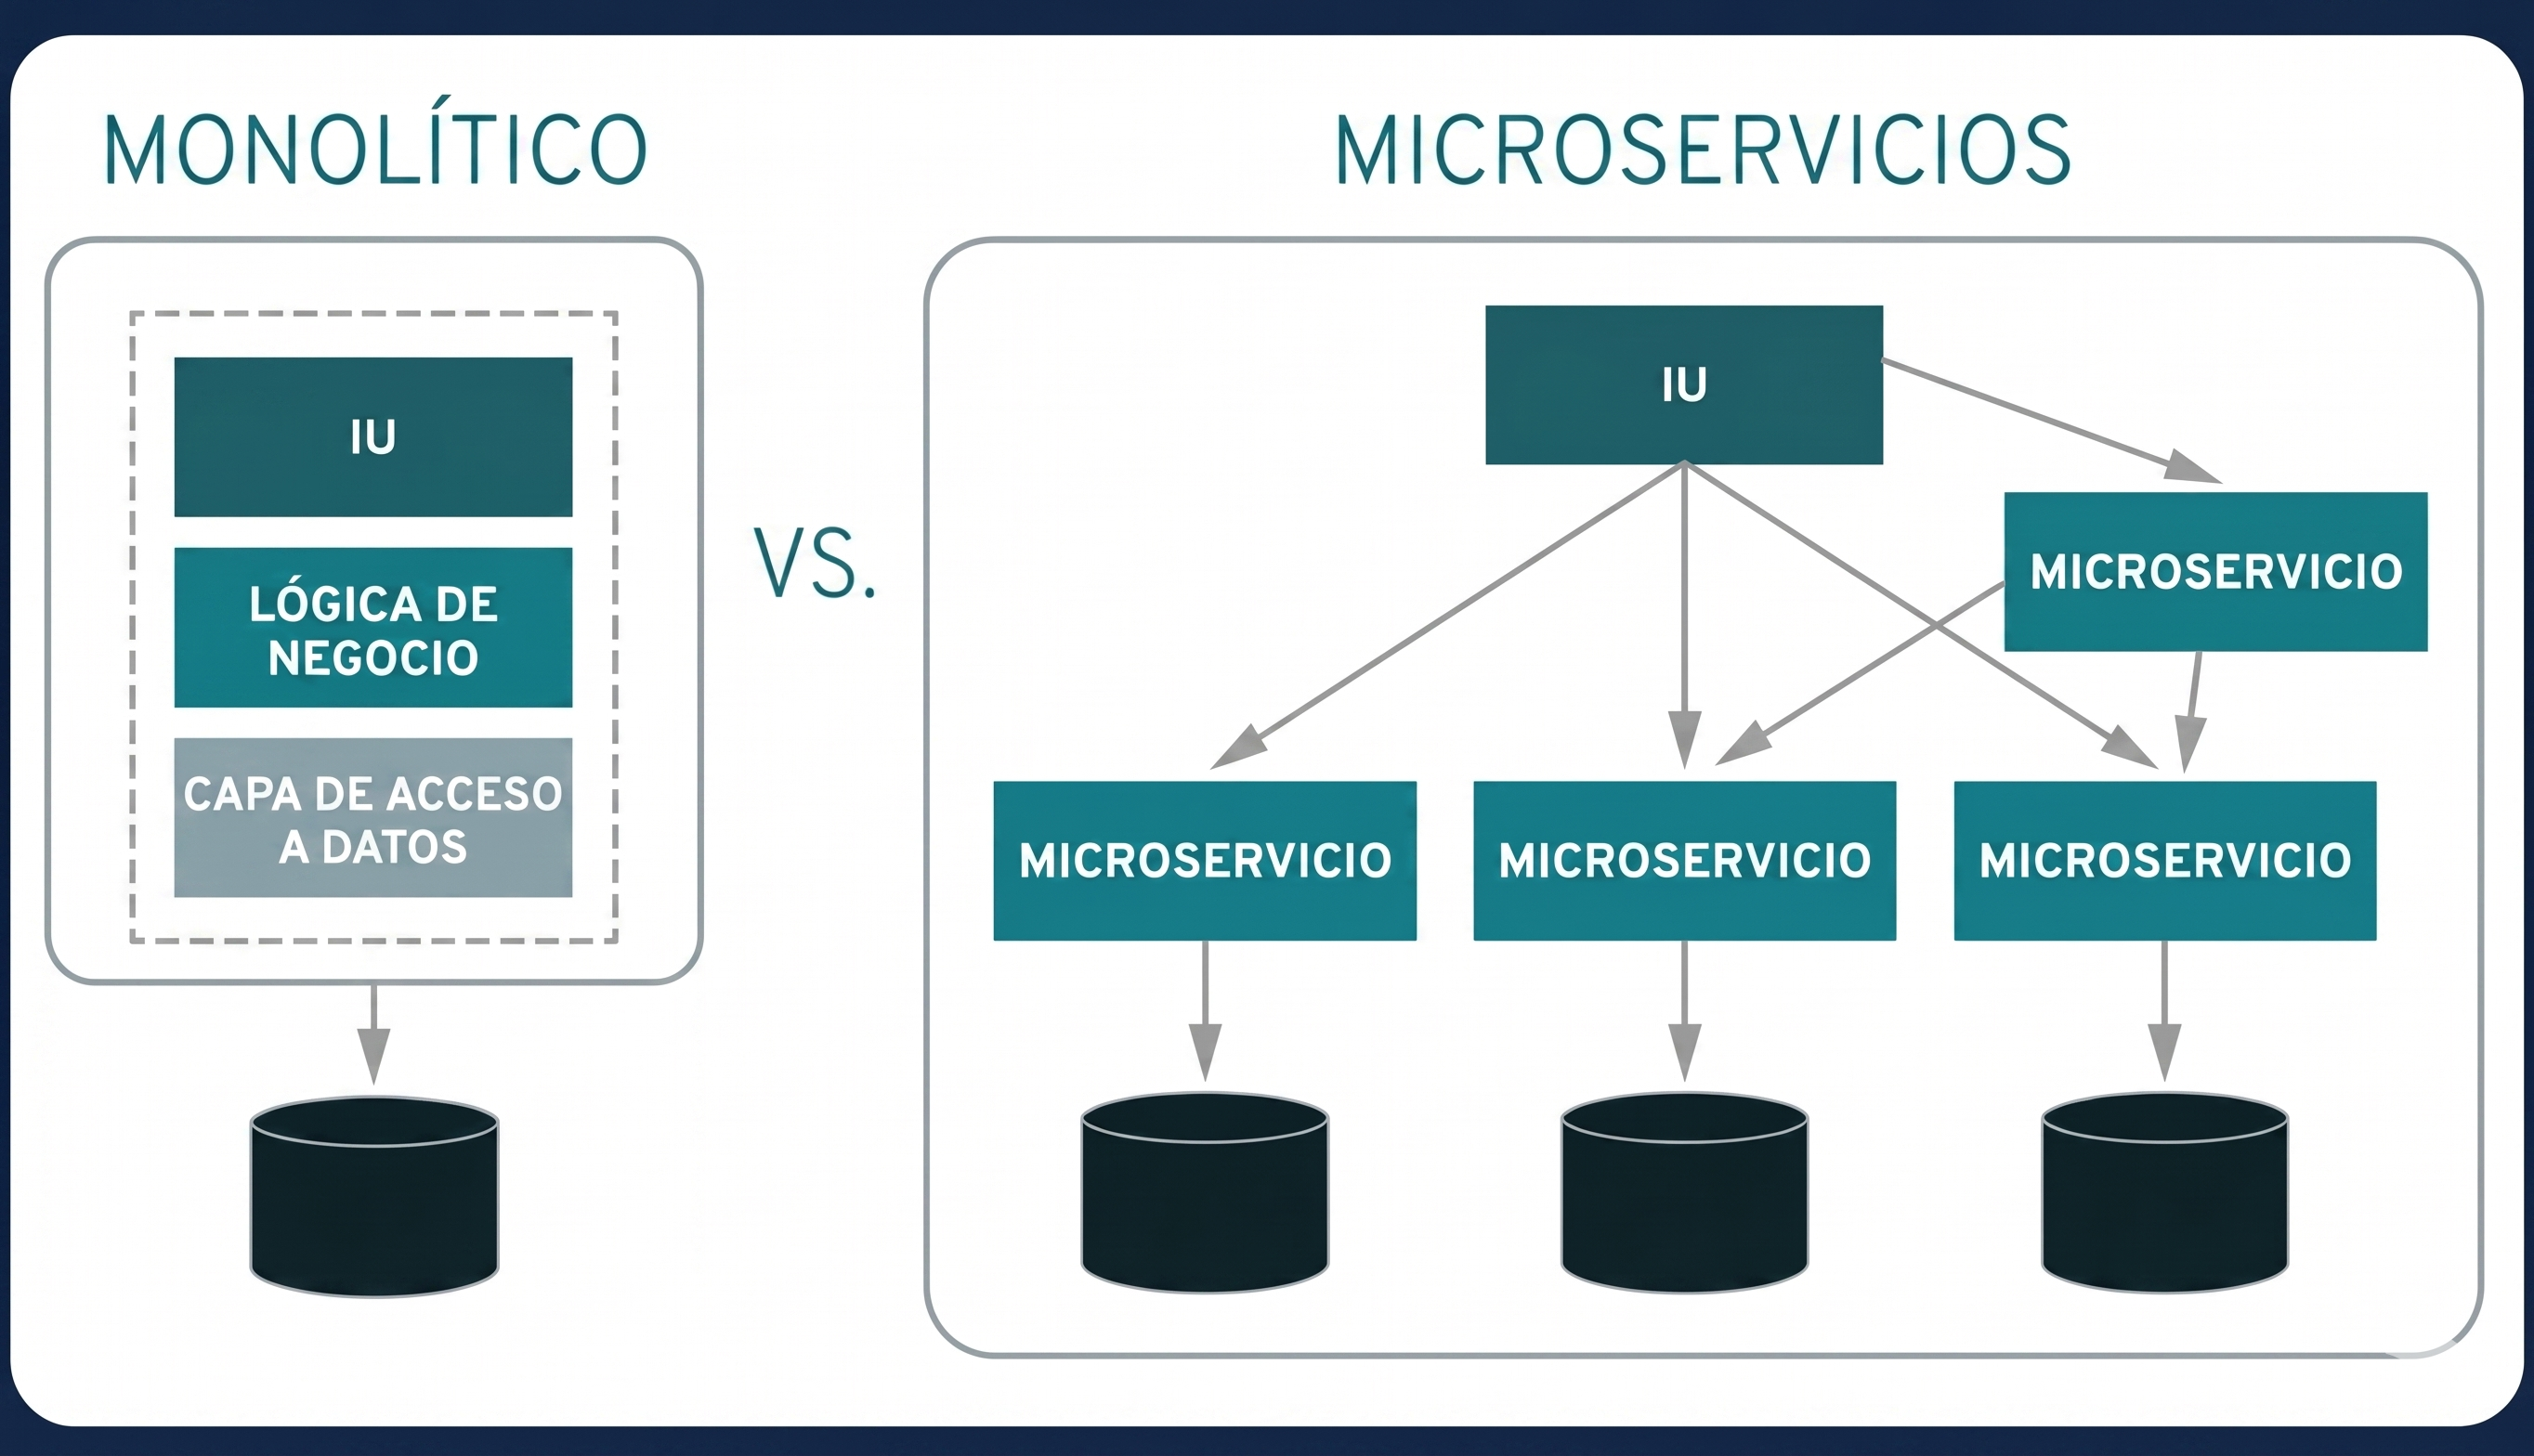
\includegraphics[width=0.7\textwidth]{imagenes/documento/arquitecturademicroservicios.png}
    \caption{Comunicación entre microservicios.}
    \label{fig:microservicios}
\end{figure}

Cada microservicio posee sus propios procesos de ejecución, mecanismos de persistencia y lógica de negocio, permitiendo implementar despliegues independientes y estrategias de escalabilidad específicas para cada componente. Esta característica resulta especialmente útil en sistemas distribuidos con cargas variables y requisitos de alta disponibilidad.

Entre las principales características de esta arquitectura destacan:

\begin{itemize}
\item \textbf{Autonomía funcional:} Cada servicio puede desarrollarse, desplegarse y mantenerse de forma independiente.

\item \textbf{Desacoplamiento:} La separación de responsabilidades reduce la dependencia entre módulos y facilita la evolución tecnológica.

\item \textbf{Escalabilidad independiente:} Los servicios pueden escalar horizontalmente según la demanda específica de procesamiento.

\item \textbf{Resiliencia operativa:} Un fallo en un servicio no necesariamente compromete el funcionamiento global del sistema.

\item \textbf{Interoperabilidad:} Permite integrar tecnologías heterogéneas mediante protocolos estándar de comunicación.
\end{itemize}

La principal ventaja de este modelo radica en la capacidad de construir sistemas altamente flexibles y escalables. Asimismo, facilita los ciclos de integración y despliegue continuo, permitiendo actualizar componentes individuales sin afectar el funcionamiento general de la aplicación \cite{32}.

No obstante, la arquitectura de microservicios también introduce desafíos relacionados con la complejidad operativa, la observabilidad distribuida, la gestión de redes, la sincronización de datos y el monitoreo de servicios. Debido a ello, su implementación suele requerir herramientas complementarias para el descubrimiento de servicios, balanceo de carga y tolerancia a fallos \cite{32}.

\subsection{Arquitectura de tres capas}

La arquitectura de tres capas es un modelo de organización de software que divide una aplicación en tres niveles lógicos independientes: presentación, lógica de negocio y persistencia de datos. Su propósito principal consiste en separar responsabilidades para reducir el acoplamiento entre componentes y facilitar el mantenimiento del sistema \cite{33}.

Este patrón arquitectónico es ampliamente utilizado en aplicaciones empresariales debido a que permite estructurar los procesos internos de manera organizada y modular. Cada capa interactúa únicamente con las capas adyacentes, favoreciendo la reutilización de componentes y la claridad estructural del sistema.

\begin{figure}[H]
    \centering
    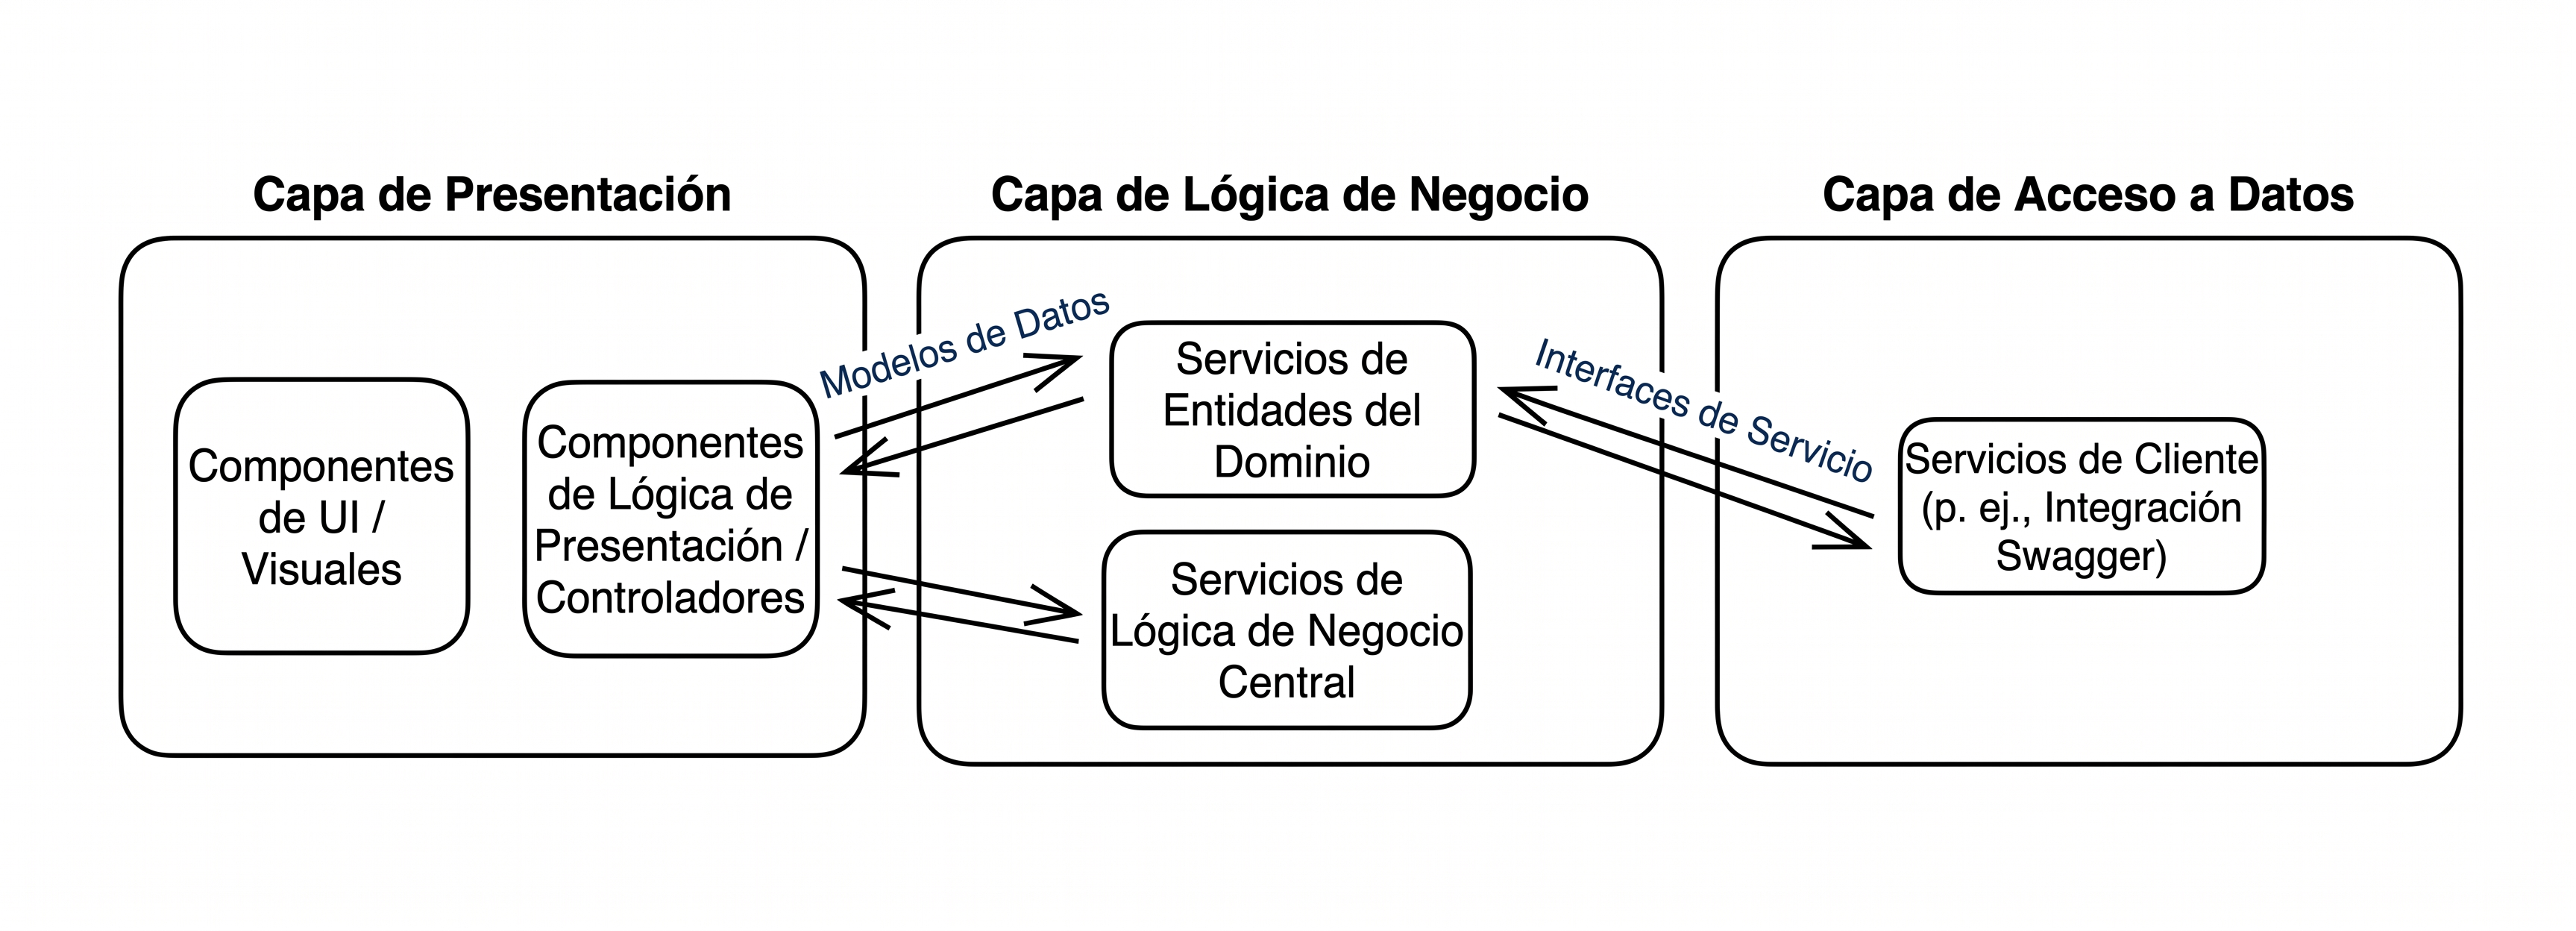
\includegraphics[width=0.7\textwidth]{imagenes/documento/patron3capas.png}
    \caption{Patrón de arquitectura de tres capas.}
    \label{fig:patron3capas}
\end{figure}

Las capas que conforman esta arquitectura son las siguientes:

\begin{itemize}

\item \textbf{Capa de presentación:} Encargada de la interacción con el usuario o con sistemas externos. Su función consiste en recibir solicitudes, mostrar información y transmitir datos hacia la lógica de negocio.

\item \textbf{Capa de lógica de negocio:} Constituye el núcleo funcional de la aplicación. En esta capa se implementan las reglas, validaciones y procesos que definen el comportamiento del sistema.

\item \textbf{Capa de persistencia:} Responsable de la comunicación con los sistemas de almacenamiento de datos. Gestiona operaciones de acceso, recuperación y almacenamiento de información.
\end{itemize}

La separación estructural proporcionada por este modelo mejora significativamente la mantenibilidad y escalabilidad de las aplicaciones, ya que cada capa puede modificarse o evolucionar con un impacto mínimo sobre las demás \cite{40}.

Sin embargo, una segmentación excesiva también puede incrementar la complejidad del sistema y generar sobrecarga en la comunicación entre capas cuando no se diseña adecuadamente \cite{40}.

\subsection{Servidor web (NGINX)}

NGINX es un software de código abierto utilizado como servidor web, balanceador de carga y gestor de contenido estático. Su arquitectura basada en eventos y procesamiento asíncrono le permite manejar un gran número de conexiones concurrentes con un consumo reducido de memoria y recursos del sistema.

A diferencia de los servidores tradicionales basados en procesos o hilos por conexión, NGINX emplea un modelo no bloqueante orientado a eventos, lo que mejora considerablemente el rendimiento bajo escenarios de alta concurrencia.

Dentro de arquitecturas distribuidas y ecosistemas de microservicios, NGINX suele utilizarse como punto de entrada centralizado para gestionar el tráfico de red y redirigir solicitudes hacia los servicios internos correspondientes.

Entre sus principales funcionalidades destacan:

\begin{itemize}

\item \textbf{Balanceo de carga:} Distribuye solicitudes entre distintas instancias de servicios para mejorar la disponibilidad y el rendimiento.

\item \textbf{Caché de contenido:} Reduce tiempos de respuesta mediante almacenamiento temporal de recursos frecuentes.

\item \textbf{Gestión de tráfico concurrente:} Permite atender miles de conexiones simultáneas con alta eficiencia.
\end{itemize}

En arquitecturas modernas, NGINX también puede implementar el patrón \textit{API Gateway}, actuando como intermediario entre clientes y servicios internos mediante mecanismos de autenticación, control de acceso y enrutamiento dinámico.

\section{Tecnologías de Desarrollo}

\subsection{Lenguaje de programación: Java}

Java es un lenguaje de programación orientado a objetos ampliamente utilizado en sistemas empresariales y aplicaciones distribuidas debido a su portabilidad, robustez y seguridad, permitiendo ejecutar aplicaciones sobre múltiples plataformas mediante la Java Virtual Machine (JVM).

La JVM actúa como una capa de abstracción entre el sistema operativo y el código compilado, proporcionando independencia de plataforma y mecanismos automáticos de administración de memoria. Esta arquitectura favorece la estabilidad y confiabilidad de aplicaciones de gran escala.

Entre las principales características técnicas de Java destacan:

\begin{itemize}
\item \textbf{Tipado fuerte:} Reduce errores durante la compilación y mejora la seguridad del código.

\item \textbf{Gestión automática de memoria:} El recolector de basura administra dinámicamente la memoria utilizada por la aplicación.

\item \textbf{Soporte multihilo:} Facilita el procesamiento concurrente y la ejecución paralela de tareas.

\item \textbf{Portabilidad:} Las aplicaciones pueden ejecutarse en diferentes sistemas operativos sin modificaciones adicionales.

\item \textbf{Amplio ecosistema empresarial:} Posee una gran cantidad de frameworks y herramientas para el desarrollo de sistemas distribuidos.
\end{itemize}

Debido a estas características, Java se ha consolidado como una de las tecnologías más utilizadas para aplicaciones backend de alta disponibilidad y arquitecturas empresariales distribuidas.

\subsection{Framework: Spring Boot}

Spring Boot es un framework perteneciente al ecosistema Spring orientado al desarrollo de aplicaciones empresariales y microservicios. Su principal objetivo consiste en simplificar la configuración y despliegue de aplicaciones Java mediante mecanismos de configuración automática y convenciones predefinidas \cite{38}.

Este framework adopta el principio \textit{Convention over Configuration}, reduciendo significativamente la complejidad asociada a la configuración manual de componentes y dependencias.

Entre sus principales características destacan:

\begin{itemize}
\item \textbf{Configuración automática:} Detecta dependencias y configura componentes automáticamente según el entorno de ejecución.

\item \textbf{Servidores embebidos:} Permite ejecutar aplicaciones sin necesidad de desplegar manualmente servidores externos.

\item \textbf{Integración modular:} Facilita la incorporación de tecnologías de persistencia, seguridad y comunicación distribuida.

\item \textbf{Desarrollo de APIs REST:} Proporciona herramientas para la construcción de servicios web y arquitecturas distribuidas.

\item \textbf{Compatibilidad con Spring Ecosystem:} Permite integrar módulos especializados como Spring Security, Spring Data y Spring Cloud.
\end{itemize}

El núcleo conceptual del framework se fundamenta en los principios de Inversión de Control (IoC) e Inyección de Dependencias (DI), los cuales delegan la creación y administración de objetos al contenedor de Spring, reduciendo el acoplamiento entre componentes.

\subsubsection{Spring Boot Actuator}

Spring Boot Actuator es un módulo orientado a la observabilidad y monitoreo de aplicaciones en entornos de producción. Proporciona mecanismos para inspeccionar métricas, estados internos y comportamiento operativo de una aplicación sin necesidad de desarrollar herramientas adicionales \cite{51}.

Entre las funcionalidades más relevantes se encuentran:

\begin{itemize}
\item Supervisión del estado de salud de la aplicación.
\item Exposición de métricas de rendimiento.
\item Monitoreo del consumo de memoria y CPU.
\item Gestión dinámica de registros de eventos (\textit{logs}).
\item Inspección de componentes internos administrados por Spring.
\end{itemize}

\begin{figure}[htbp]
    \centering
    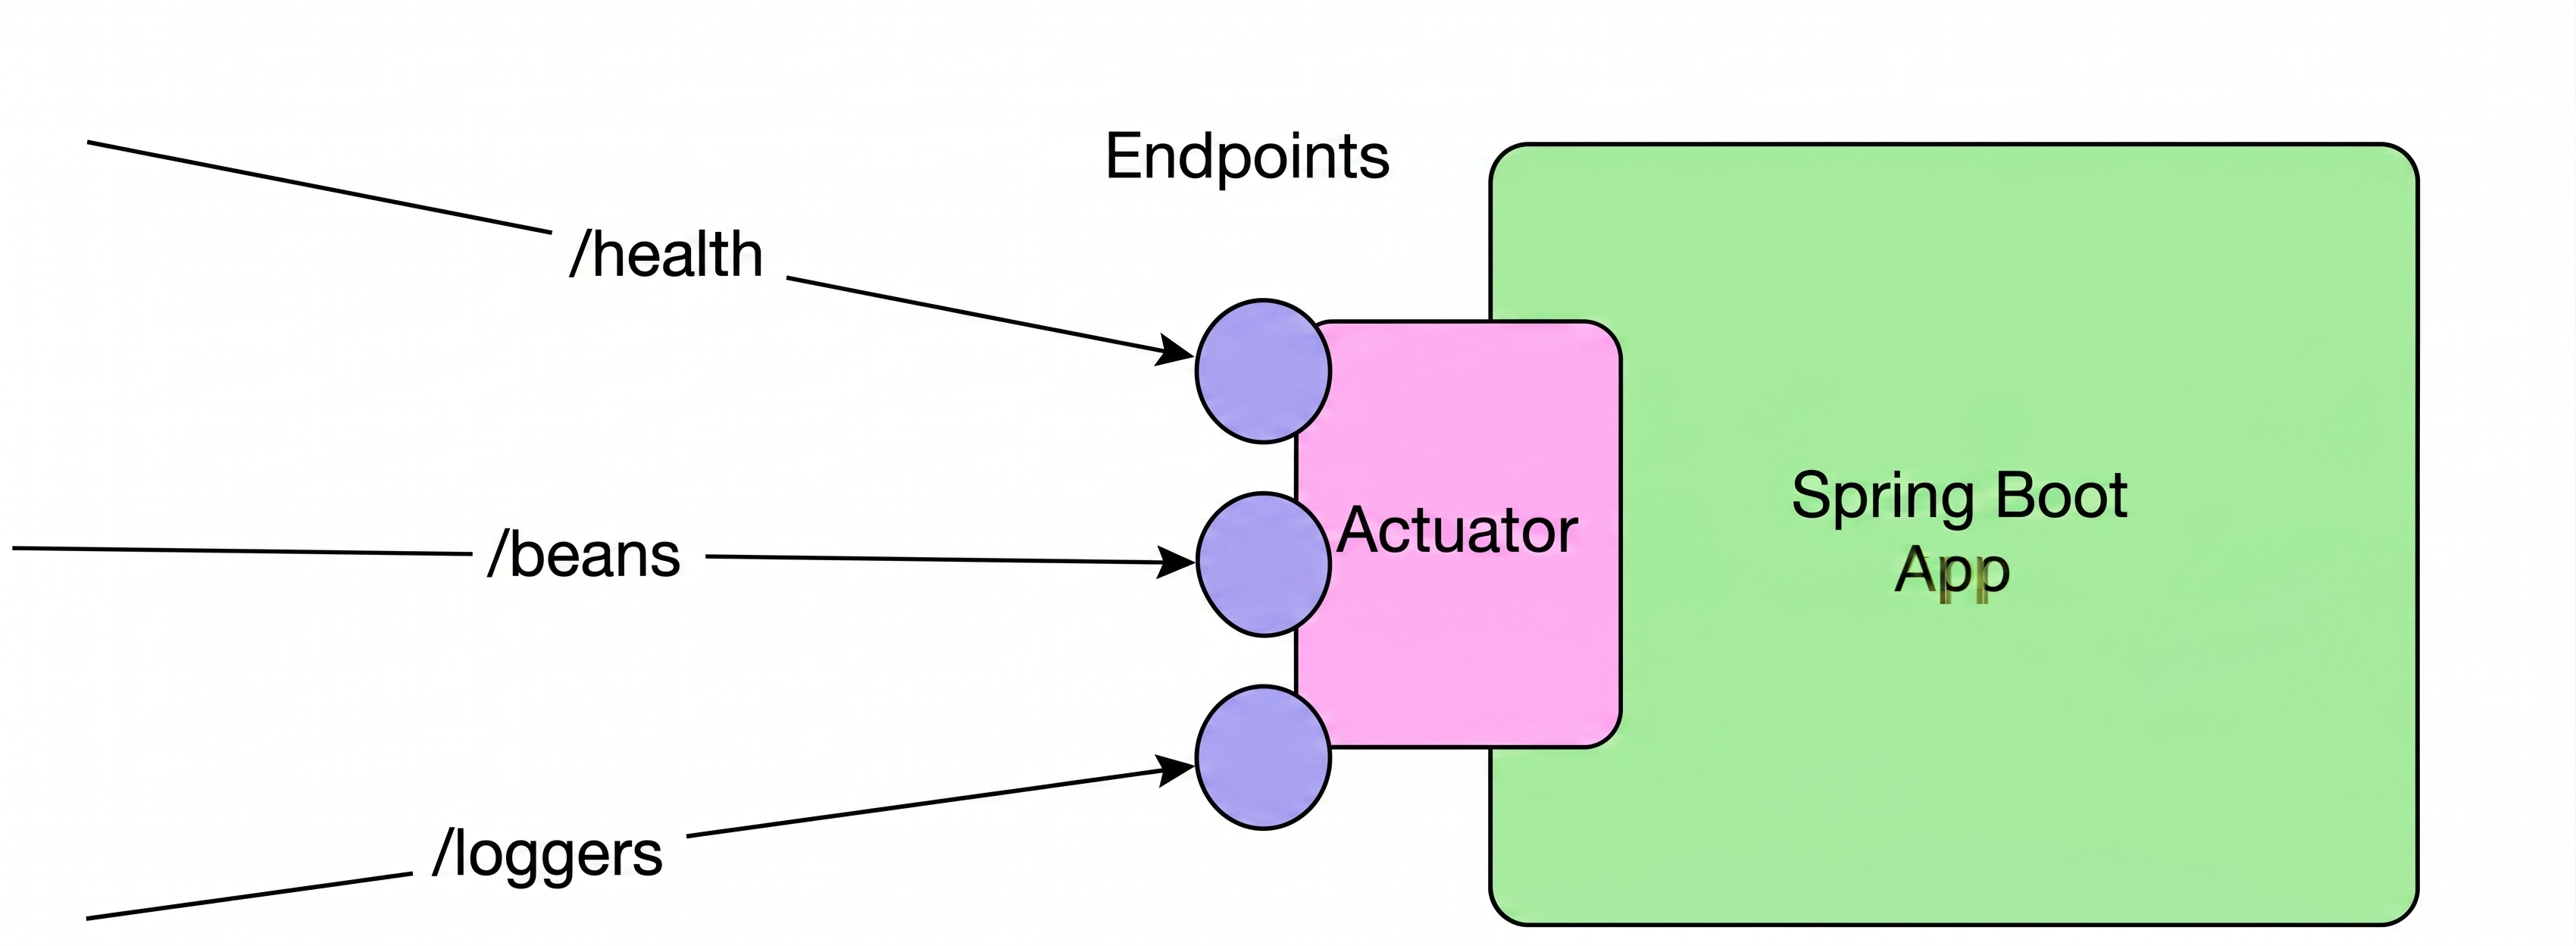
\includegraphics[width=0.8\textwidth]{imagenes/documento/actuador.png}
    \caption{Endpoints de monitoreo proporcionados por Spring Boot Actuator.}
    \label{fig:spring_actuator_endpoints}
\end{figure}

Estas capacidades permiten mejorar la observabilidad del sistema y facilitan la detección temprana de errores dentro de entornos distribuidos.

\subsubsection{Spring Security y JWT}

Spring Security es un framework especializado en autenticación y autorización para aplicaciones Java. Su objetivo principal consiste en proteger recursos mediante mecanismos de control de acceso, validación de identidad y gestión de permisos.

Dentro de arquitecturas modernas distribuidas, es común utilizar estándares como JWT (\textit{JSON Web Tokens}) para implementar autenticación basada en tokens \cite{52}.

JWT es un estándar de representación compacta de información firmado digitalmente, utilizado para transportar datos de autenticación y autorización entre sistemas.

El funcionamiento general del esquema basado en JWT consiste en:

\begin{enumerate}
\item El usuario se autentica mediante credenciales válidas.
\item El servidor genera un token firmado digitalmente.
\item El cliente almacena el token y lo envía en cada solicitud.
\item El servidor valida la autenticidad y vigencia del token antes de permitir el acceso.
\end{enumerate}

Este enfoque permite construir sistemas \textit{stateless}, reduciendo la dependencia de sesiones persistentes y facilitando la escalabilidad horizontal en arquitecturas distribuidas.

No obstante, el uso de JWT también introduce desafíos relacionados con la revocación de tokens, el manejo seguro de claves criptográficas y la protección contra ataques de reutilización de credenciales.

\subsubsection{Spring Cloud: Configuración distribuida y descubrimiento de servicios}

Spring Cloud es un conjunto de herramientas orientadas al desarrollo de sistemas distribuidos y arquitecturas basadas en microservicios. Su propósito consiste en proporcionar soluciones para problemas comunes en entornos distribuidos, tales como configuración centralizada, descubrimiento de servicios, balanceo de carga y tolerancia a fallos \cite{53}.

\paragraph{Configuración centralizada}

En sistemas distribuidos, mantener configuraciones independientes para cada servicio puede generar inconsistencias y dificultades de mantenimiento. Para resolver este problema, Spring Cloud Config permite centralizar propiedades y parámetros de configuración dentro de repositorios externos.

Este enfoque facilita la administración de múltiples entornos de ejecución, permitiendo separar configuraciones de desarrollo, pruebas y producción. Asimismo, favorece la actualización dinámica de parámetros sin necesidad de modificar directamente el código fuente de los servicios.

\paragraph{Descubrimiento de servicios}

Dentro de arquitecturas basadas en microservicios, las instancias pueden crearse, eliminarse o modificarse dinámicamente. Debido a ello, resulta necesario implementar mecanismos automáticos de localización de servicios.

Spring Cloud integra herramientas de \textit{Service Discovery}, las cuales permiten registrar servicios dentro de un directorio centralizado. Los clientes pueden localizar servicios mediante nombres lógicos en lugar de depender de direcciones IP estáticas.

Entre las principales ventajas de este modelo destacan:

\begin{itemize}
\item Descubrimiento automático de servicios.
\item Balanceo dinámico de carga.
\item Reducción del acoplamiento entre componentes.
\item Mayor tolerancia a fallos en sistemas distribuidos.
\item Simplificación de la comunicación entre servicios.
\end{itemize}

No obstante, este tipo de arquitecturas también introduce complejidad adicional relacionada con la sincronización de estados, monitoreo distribuido y administración de infraestructura.

\subsection{Interfaces de Programación de Aplicaciones (API REST)}

Las Interfaces de Programación de Aplicaciones bajo el estilo arquitectónico REST (\textit{Representational State Transfer}) constituyen uno de los modelos de comunicación más utilizados en sistemas distribuidos y arquitecturas basadas en servicios \cite{54}.

REST define un conjunto de principios para la transferencia de recursos mediante protocolos estándar de la web, particularmente HTTP. En este enfoque, cada recurso posee una dirección única identificada mediante una URI y puede manipularse utilizando operaciones HTTP como GET, POST, PUT y DELETE.

Entre las principales características de las APIs REST destacan:

\begin{itemize}
\item \textbf{Comunicación sin estado (\textit{stateless}):} Cada solicitud contiene toda la información necesaria para ser procesada.

\item \textbf{Interoperabilidad:} Facilita la comunicación entre sistemas heterogéneos mediante estándares abiertos.

\item \textbf{Escalabilidad:} La ausencia de sesiones persistentes mejora el manejo de múltiples solicitudes concurrentes.

\item \textbf{Separación cliente-servidor:} Permite desacoplar interfaces de usuario y servicios backend.

\item \textbf{Uso de formatos estándar:} Generalmente emplea JSON o XML para el intercambio de información.
\end{itemize}

En arquitecturas modernas, las APIs REST suelen complementarse con estrategias de versionamiento para mantener compatibilidad entre distintas versiones de servicios. Asimismo, es común implementar mecanismos de control de tráfico (\textit{Rate Limiting}) con el objetivo de evitar saturación y abuso de recursos.

\subsection{Protocolos de Transporte Seguro: TLS 1.3}

TLS (\textit{Transport Layer Security}) es un protocolo criptográfico diseñado para garantizar confidencialidad, integridad y autenticación en comunicaciones realizadas a través de redes informáticas \cite{55}.

La versión TLS 1.3 representa una evolución significativa respecto a versiones anteriores, incorporando mejoras relacionadas con seguridad y rendimiento. Entre sus principales características destacan:

\begin{itemize}
\item \textbf{Reducción de latencia:} Optimiza el proceso de establecimiento de conexión mediante un menor número de intercambios durante el \textit{handshake}.

\item \textbf{Eliminación de algoritmos inseguros:} Suprime mecanismos criptográficos obsoletos o vulnerables presentes en versiones anteriores.

\item \textbf{Perfect Forward Secrecy (PFS):} Garantiza que la exposición futura de claves privadas no comprometa comunicaciones previas.

\item \textbf{Cifrado autenticado:} Utiliza algoritmos AEAD (\textit{Authenticated Encryption with Associated Data}) para proteger confidencialidad e integridad simultáneamente.
\end{itemize}

Una de las mejoras más importantes de TLS 1.3 consiste en la reducción de la latencia durante el establecimiento de conexiones seguras mediante mecanismos como 1-RTT y 0-RTT \cite{56}.

No obstante, la implementación de protocolos criptográficos modernos también requiere una administración adecuada de certificados digitales, políticas de seguridad y actualización constante de dependencias criptográficas.

\subsection{Resiliencia del Sistema: API Gateway}

La resiliencia en sistemas distribuidos se refiere a la capacidad de una arquitectura para mantener su funcionamiento ante fallos parciales, interrupciones de red o sobrecarga de servicios \cite{58}.

Dentro de arquitecturas basadas en microservicios, es común implementar patrones especializados para mejorar la tolerancia a fallos y reducir el impacto de errores distribuidos.

\paragraph{API Gateway}

El patrón API Gateway actúa como un punto de entrada centralizado para las solicitudes realizadas por los clientes. Este componente abstrae la complejidad interna del sistema y centraliza funcionalidades como autenticación, balanceo de carga, monitoreo y enrutamiento dinámico.

Entre sus principales ventajas destacan:

\begin{itemize}
\item Simplificación de la comunicación cliente-servidor.
\item Centralización de políticas de seguridad.
\item Ocultamiento de la topología interna.
\item Control unificado del tráfico de red.
\item Integración de mecanismos de monitoreo y filtrado.
\end{itemize}

\section{Infraestructura y Orquestación}

La infraestructura computacional moderna se fundamenta en mecanismos de abstracción y virtualización que permiten optimizar el uso de recursos físicos, mejorar la portabilidad de las aplicaciones y facilitar la administración de entornos distribuidos. En arquitecturas basadas en microservicios, la infraestructura debe ser capaz de soportar despliegues dinámicos, escalabilidad horizontal y recuperación automática ante fallos.

Dentro de este contexto, tecnologías como la virtualización, la contenerización y la orquestación de contenedores constituyen elementos fundamentales para la construcción de sistemas distribuidos de alta disponibilidad.
\begin{figure}[htbp]
    \centering
    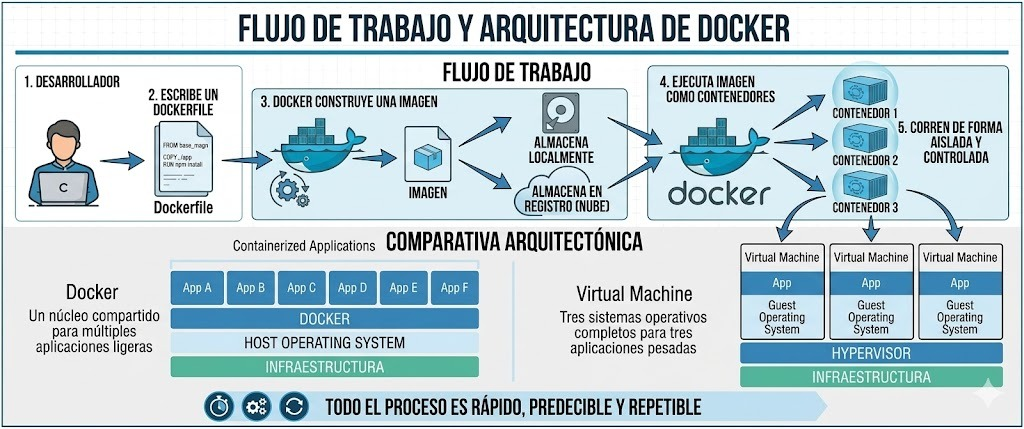
\includegraphics[width=0.8\textwidth]{imagenes/documento/docker.png}
    \caption{Funcionamiento de Docker y Kubernetes en la infraestructura de microservicios.}
    \label{fig:docker_kubernetes}
\end{figure}

\subsection{Virtualización e Hipervisores}

La virtualización es una técnica computacional que permite ejecutar múltiples entornos aislados sobre una misma infraestructura física mediante la abstracción del hardware subyacente. Este enfoque incrementa el aprovechamiento de recursos y facilita la administración de servidores y aplicaciones.

El componente principal encargado de gestionar este proceso es el \textbf{hipervisor} (\textit{Hypervisor}), una capa de software especializada que administra el acceso al hardware físico y permite crear y ejecutar múltiples máquinas virtuales de manera simultánea.

Existen dos categorías principales de hipervisores:

\begin{itemize}
\item \textbf{Hipervisores Tipo 1 (Bare Metal):} Se ejecutan directamente sobre el hardware físico sin requerir un sistema operativo anfitrión. Ejemplos comunes incluyen VMware ESXi, Xen y Microsoft Hyper-V.

\item \textbf{Hipervisores Tipo 2 (Hosted):} Operan sobre un sistema operativo anfitrión, utilizando sus recursos para ejecutar máquinas virtuales. Entre los más utilizados se encuentran VirtualBox y VMware Workstation.
\end{itemize}

La virtualización proporciona ventajas importantes relacionadas con aislamiento, consolidación de servidores y flexibilidad operativa. Sin embargo, las máquinas virtuales suelen requerir una mayor cantidad de recursos debido a que cada instancia incorpora un sistema operativo completo.

\subsection{Máquinas Virtuales y Sistema Operativo Anfitrión}

Una \textbf{máquina virtual} (\textit{Virtual Machine}) es una representación virtualizada de un sistema computacional completo, incluyendo procesador, memoria, almacenamiento y sistema operativo. Cada máquina virtual opera de manera aislada respecto a las demás, como si se tratara de un equipo físico independiente.

Dentro de este modelo intervienen dos conceptos fundamentales:

\begin{itemize}
\item \textbf{Host Operating System:} Sistema operativo anfitrión encargado de administrar directamente el hardware físico del servidor o estación de trabajo.

\item \textbf{Guest Operating System:} Sistema operativo invitado que se ejecuta dentro de una máquina virtual mediante la capa de virtualización proporcionada por el hipervisor.
\end{itemize}

Este enfoque permite ejecutar múltiples sistemas operativos simultáneamente sobre un mismo hardware físico, facilitando tareas de desarrollo, pruebas, consolidación de infraestructura y despliegue de servicios distribuidos.

No obstante, debido a que cada máquina virtual incorpora su propio núcleo del sistema operativo y recursos dedicados, el consumo de memoria y procesamiento puede incrementarse significativamente en comparación con otras alternativas más ligeras.

\subsection{Contenerización}

La contenerización es un modelo de virtualización ligera que permite empaquetar aplicaciones junto con sus dependencias, librerías y configuraciones necesarias para su ejecución dentro de unidades aisladas denominadas contenedores.

A diferencia de las máquinas virtuales tradicionales, los contenedores no requieren un sistema operativo completo para cada instancia. En su lugar, comparten el núcleo del sistema operativo anfitrión, reduciendo significativamente el consumo de recursos y mejorando los tiempos de despliegue.

Este modelo proporciona ventajas importantes relacionadas con:

\begin{itemize}
\item Portabilidad entre entornos.
\item Aislamiento de aplicaciones.
\item Reproducibilidad de configuraciones.
\item Escalabilidad rápida.
\item Reducción del consumo de infraestructura.
\end{itemize}

La contenerización se ha convertido en uno de los pilares fundamentales de las arquitecturas basadas en microservicios debido a su capacidad para simplificar despliegues distribuidos y mantener consistencia entre entornos de desarrollo, pruebas y producción.

\subsection{Docker}

Docker es una plataforma de código abierto orientada a la creación, distribución y ejecución de contenedores \cite{58}. Su arquitectura permite encapsular aplicaciones junto con todas sus dependencias dentro de entornos aislados y portables.

El funcionamiento de Docker se basa en tecnologías del núcleo de Linux como \textit{Namespaces} y \textit{Control Groups (cgroups)}, las cuales permiten aislar procesos y controlar el consumo de recursos de cada contenedor.

Entre los principales componentes del ecosistema Docker destacan:

\begin{itemize}

\item \textbf{Docker Engine:} Motor principal encargado de construir y ejecutar contenedores.

\item \textbf{Dockerfile:} Archivo declarativo que contiene las instrucciones necesarias para construir imágenes de contenedores.

\item \textbf{Imágenes:} Plantillas inmutables que incluyen dependencias, librerías y configuraciones requeridas para ejecutar aplicaciones.

\item \textbf{Contenedores:} Instancias ejecutables creadas a partir de imágenes Docker.

\item \textbf{Docker Registry:} Repositorio utilizado para almacenar y distribuir imágenes.

\item \textbf{Docker Compose:} Herramienta destinada a definir y administrar aplicaciones compuestas por múltiples contenedores.
\end{itemize}

Una de las principales ventajas de Docker consiste en garantizar consistencia operativa entre diferentes entornos de ejecución. Esto permite que una aplicación pueda ejecutarse de manera idéntica independientemente de la infraestructura subyacente.

Sin embargo, el uso masivo de contenedores también introduce desafíos relacionados con monitoreo, seguridad, redes distribuidas y administración de múltiples servicios concurrentes.

\subsection{Orquestación de Contenedores con Kubernetes}

Kubernetes es una plataforma de código abierto diseñada para automatizar el despliegue, administración y escalabilidad de aplicaciones contenerizadas \cite{59}.

Su principal objetivo consiste en coordinar múltiples contenedores distribuidos dentro de un clúster computacional, garantizando disponibilidad, balanceo de carga y recuperación automática ante fallos.

Kubernetes implementa un modelo declarativo de infraestructura, donde el usuario define el estado deseado del sistema y la plataforma se encarga automáticamente de mantener dicha configuración.

Entre las principales abstracciones utilizadas por Kubernetes destacan:

\begin{itemize}

\item \textbf{Pods:} Unidad mínima de ejecución que agrupa uno o más contenedores relacionados.

\item \textbf{Deployments:} Recursos encargados de administrar el estado deseado de las aplicaciones y sus actualizaciones.

\item \textbf{Services:} Componentes que proporcionan conectividad y balanceo de carga entre Pods.

\item \textbf{Namespaces:} Mecanismos de aislamiento lógico dentro del clúster.

\item \textbf{Horizontal Pod Autoscaler (HPA):} Sistema de escalabilidad automática basado en métricas de utilización.
\end{itemize}

Además de la orquestación de contenedores, Kubernetes incorpora funcionalidades relacionadas con:

\begin{itemize}
\item Recuperación automática ante fallos.
\item Distribución dinámica de tráfico.
\item Escalabilidad horizontal.
\item Gestión declarativa de infraestructura.
\item Monitoreo y supervisión de servicios.
\item Balanceo de carga distribuido.
\end{itemize}

Estas capacidades convierten a Kubernetes en una de las principales plataformas para la administración de infraestructuras modernas basadas en microservicios y computación distribuida.

No obstante, la administración de clústeres distribuidos también introduce complejidad significativa relacionada con redes, observabilidad, seguridad, almacenamiento persistente y consumo de recursos computacionales.

\section{Gestión de Bases de Datos}

La gestión de bases de datos constituye uno de los componentes fundamentales dentro de los sistemas distribuidos modernos, ya que permite almacenar, organizar, consultar y proteger grandes volúmenes de información de manera eficiente. 

En arquitecturas basadas en microservicios, los sistemas gestores de bases de datos deben garantizar propiedades relacionadas con integridad, concurrencia, disponibilidad, seguridad y escalabilidad, permitiendo que múltiples servicios interactúen simultáneamente sobre los datos sin comprometer su consistencia.

\subsection{PostgreSQL}

PostgreSQL es un sistema de gestión de bases de datos relacional orientado a objetos (\textit{Object Relational Database Management System, ORDBMS}) de código abierto, ampliamente reconocido por su robustez, estabilidad y cumplimiento de estándares SQL \cite{42}.

Su arquitectura permite combinar características tradicionales de los sistemas relacionales con capacidades avanzadas orientadas al manejo de datos complejos y aplicaciones distribuidas.

A diferencia de motores ligeros enfocados únicamente en almacenamiento relacional básico, PostgreSQL incorpora mecanismos avanzados de concurrencia, indexación, recuperación ante fallos y extensibilidad, lo que lo convierte en una solución ampliamente utilizada en aplicaciones empresariales, plataformas web y sistemas de misión crítica.

Entre sus principales características destacan:

\begin{itemize}

\item \textbf{Cumplimiento de propiedades ACID:} Garantiza atomicidad, consistencia, aislamiento y durabilidad en las transacciones, asegurando que las operaciones sobre los datos se ejecuten de forma íntegra y confiable.

\item \textbf{Control de concurrencia multiversión (MVCC):} Permite que múltiples transacciones accedan simultáneamente a la información sin bloquear completamente las tablas, mejorando el rendimiento en entornos concurrentes.

\item \textbf{Soporte para transacciones complejas:} Incluye subconsultas, procedimientos almacenados, disparadores (\textit{triggers}) y operaciones avanzadas de manipulación de datos.

\item \textbf{Extensibilidad:} Permite incorporar tipos de datos personalizados, funciones definidas por el usuario y extensiones adicionales.

\item \textbf{Compatibilidad con múltiples índices avanzados:} Soporta estructuras de indexación como B-Tree, Hash, GiST y GIN.

\item \textbf{Soporte híbrido de datos:} Permite trabajar tanto con modelos relacionales tradicionales como con datos semi-estructurados mediante JSON y JSONB.
\end{itemize}

Gracias a estas capacidades, PostgreSQL se ha consolidado como uno de los sistemas gestores de bases de datos más utilizados en arquitecturas modernas que requieren alta integridad, confiabilidad y capacidad de procesamiento concurrente.

\subsection{Manejo de datos semi-estructurados mediante JSONB}

Los sistemas actuales generan grandes cantidades de información cuya estructura puede variar dinámicamente dependiendo del contexto de la aplicación. Para responder a esta necesidad, PostgreSQL incorpora soporte para datos semi-estructurados mediante los tipos JSON y JSONB.

El tipo \textbf{JSONB} (\textit{JSON Binary}) almacena documentos JSON en un formato binario optimizado, permitiendo realizar búsquedas, filtrados e indexación de manera más eficiente que el tipo JSON convencional \cite{60}.

A diferencia del almacenamiento textual tradicional, JSONB descompone internamente la estructura del documento, facilitando operaciones de consulta y acceso rápido a los atributos almacenados.

Entre las principales ventajas de JSONB destacan:

\begin{itemize}

\item \textbf{Flexibilidad en el modelado de datos:} Permite almacenar estructuras dinámicas sin necesidad de modificar constantemente el esquema relacional.

\item \textbf{Consultas eficientes:} Facilita búsquedas sobre atributos específicos dentro de documentos complejos.

\item \textbf{Compatibilidad con operadores especializados:} PostgreSQL incorpora operadores para validar existencia de claves, comparar estructuras y filtrar contenido interno.

\item \textbf{Integración con mecanismos avanzados de indexación:} Mejora significativamente el rendimiento en consultas sobre grandes volúmenes de documentos.
\end{itemize}

El uso de datos semi-estructurados resulta especialmente útil en sistemas que manejan metadatos variables, registros dinámicos, bitácoras, configuraciones o documentos cuyo contenido no sigue una estructura completamente rígida.

\subsection{Índices GIN y búsqueda eficiente de información}

En bases de datos con grandes volúmenes de información, las operaciones de búsqueda pueden convertirse en un cuello de botella si no existen mecanismos adecuados de indexación.

Para optimizar este tipo de consultas, PostgreSQL incorpora estructuras avanzadas conocidas como índices \textbf{GIN} (\textit{Generalized Inverted Index}) \cite{60}.

Un índice GIN funciona mediante una estructura invertida que asocia cada término, clave o elemento almacenado con las filas donde aparece dicho contenido. Este enfoque resulta especialmente eficiente para:

\begin{itemize}

\item Consultas sobre documentos JSONB.

\item Búsquedas de texto completo (\textit{Full-Text Search}).

\item Filtrado sobre arreglos y colecciones de datos.

\item Consultas sobre estructuras dinámicas o semi-estructuradas.
\end{itemize}

A diferencia de índices tradicionales como B-Tree, los índices GIN están diseñados específicamente para manejar atributos múltiples dentro de una misma estructura de datos, permitiendo acelerar considerablemente las búsquedas complejas.

Gracias a ello, PostgreSQL puede realizar consultas sobre grandes volúmenes de información textual y documental manteniendo tiempos de respuesta eficientes.

\subsection{Seguridad y cifrado de datos en reposo}

La protección de información almacenada constituye uno de los principales requisitos dentro de sistemas empresariales y aplicaciones distribuidas, especialmente cuando se gestionan datos sensibles o confidenciales.

La seguridad de datos en reposo se refiere al conjunto de mecanismos destinados a proteger la información almacenada físicamente dentro de discos, particiones o sistemas de almacenamiento persistente.

Para ello, PostgreSQL proporciona diversas estrategias relacionadas con autenticación, control de acceso y cifrado de información mediante extensiones especializadas como \texttt{pgcrypto} \cite{60}.

Entre las principales técnicas de protección destacan:

\begin{itemize}

\item \textbf{Cifrado simétrico AES-256:} Utiliza claves criptográficas para proteger información sensible mediante algoritmos de cifrado robustos y ampliamente adoptados en entornos empresariales.

\item \textbf{Funciones hash SHA-512:} Permiten generar resúmenes criptográficos únicos utilizados para verificar integridad y detectar modificaciones no autorizadas sobre los datos.

\item \textbf{Control de acceso basado en roles:} PostgreSQL implementa un modelo de permisos jerárquico que restringe operaciones según privilegios asignados a usuarios y grupos.

\item \textbf{Autenticación y políticas de acceso:} El sistema permite definir mecanismos de autenticación mediante contraseñas cifradas, certificados y reglas de acceso configurables.
\end{itemize}

Estas estrategias fortalecen la confidencialidad, integridad y disponibilidad de la información almacenada, reduciendo riesgos relacionados con accesos no autorizados y alteraciones maliciosas.

\subsection{Escalabilidad y optimización de bases de datos}

A medida que aumenta el volumen de información y el número de usuarios concurrentes, resulta necesario implementar mecanismos que permitan mantener el rendimiento y la estabilidad del sistema gestor de bases de datos.

La escalabilidad en bases de datos se refiere a la capacidad de incrementar recursos y distribuir carga de trabajo sin degradar significativamente el desempeño de las operaciones.

Entre las principales estrategias utilizadas para optimización y escalabilidad destacan:

\begin{itemize}

\item \textbf{Particionamiento de tablas (\textit{Partitioning}):} Técnica que divide grandes volúmenes de datos en segmentos más pequeños organizados por rangos, listas o criterios específicos, reduciendo tiempos de búsqueda y acceso.

\item \textbf{Pooling de conexiones:} Herramientas como \textbf{PgBouncer} permiten reutilizar conexiones activas hacia PostgreSQL, disminuyendo el costo computacional asociado a la apertura constante de nuevas conexiones.

\item \textbf{Replicación Streaming:} Permite mantener múltiples réplicas sincronizadas de una base de datos principal, mejorando disponibilidad, tolerancia a fallos y distribución de carga.

\item \textbf{Balanceo de consultas:} Las operaciones de lectura pueden distribuirse entre servidores secundarios para reducir carga sobre el nodo principal.

\item \textbf{Optimización mediante índices:} El uso adecuado de estructuras de indexación reduce significativamente el tiempo requerido para ejecutar consultas complejas.
\end{itemize}

Estas estrategias permiten incrementar la capacidad de procesamiento, mejorar la disponibilidad y mantener un comportamiento estable incluso bajo escenarios de alta demanda concurrente.